\documentclass[12pt]{article}
\usepackage[utf8]{inputenc}
\usepackage[margin=1.5in]{geometry}

\title{Properties of de Bruijn Sequences and Graphs, and a Generating Algorithm}
\author{Reed Nelson}
\date{May 2021}

\usepackage{natbib}
\usepackage{graphicx}
\usepackage{amsmath}
\usepackage{amsthm}
\usepackage{amssymb}

\newtheorem{theorem}{Theorem}[section]
\newtheorem{property}{Property}[section]
\newcounter{example}[section]
\newenvironment{example}[1][]{\refstepcounter{example}\par\medskip
   \noindent \textbf{Example~\theexample. #1} \rmfamily}{\medskip}

\renewcommand\qedsymbol{$\blacksquare$}

\begin{document}

\maketitle

\section{Introduction}
De Bruijn sequences are named after Nicolaas Govert de Bruijn, a Dutch mathematician who wrote about them in his 1946 paper \emph{A Combinatorial Problem} \citep{debruijn_1946}. The idea, however, dates back to at least the 19th century. \par
In this paper we will define what a de Bruijn sequence is, and seek to better the reader’s understanding by exploring some of their interesting combinatorial and graph theoretical properties. We will proceed to apply some of these properties in the process of developing an algorithm to generate all de Bruijn sequences for a given alphabet and window size. This algorithm will be discussed both in terms of the the broad mathematical process the algorithm uses, and in more specific terms of its practical implementation. Following that will be a brief discussion of applications of these sequences in genomics and in card magic.  


\section{Properties}
\subsection{Definition and Notation}
Let $A$ be an alphabet of $k$ distinct characters. A \emph{de Bruijn sequence} is a cyclic string of characters from $A$\footnote{A binary alphabet is often implied with de Bruijn sequences, but what this paper discusses applies for an arbitrary alphabet.}, where each permutation of $n$ characters appears exactly once. $B(k,n)$ will be used to denote the set of de Bruijn sequences of window length $n$ and alphabet length $k$.

\subsection{Basic Properties}

\begin{property}
\normalfont The length of a $B(k,n)$ sequence is $k^n$.
\end{property}
\begin{proof}
The number of n-permutations of k characters is $k^{n}$, and given by the definition, each of those permutations must appear exactly once. Take $s$ to be a minimum-length sequence of length $l$ consisting of all unique permutations in question. In each window length n sits one permutation. If the window is shifted over one character, this must give another unique permutation. Thus the smallest possible value of $l$ would be $k^{n}$. Suppose $l > k^{n}$, then the number of windows in $s$ would be greater than $k^{n}$, and thus $s$ would contain non-unique permutations, and would not be a de Bruijn sequence. Therefore, the length of a $B(k,n)$ sequence is $k^n$.
\end{proof}

\begin{property}
\normalfont The number of distinct\footnote{Because de Bruijn sequences are cyclic, we consider mere rotations of one sequence to be the same (non-distinct) sequence.} $B(k,n)$ sequences equals $\frac{(k!)^{k^{n-1}}}{k^{n}}$.
\end{property}

\begin{example}
B(2,3) \footnote{The nominal values of the characters used in the alphabet are unimportant, so for this paper and generally, when $k<10$, we take $A=\lbrace0,1,\dots,k\rbrace$.} has 2 distinct sequences, 8 characters in length:\newline 
\centerline{00010111 \hspace{5 mm} 11101000 }
\end{example}

\subsection{De Bruijn Graphs}
Each $B(k,n)$ has a corresponding de Bruijn graph. The example in Figure 1 shows the graph for $B(2,3)$.

\begin{figure}[ht!]
\centering
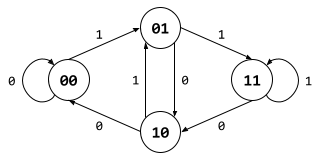
\includegraphics[scale=0.75]{graphics/b23_graph.png}
\caption{$B(2,3)$ Graph}
\label{fig:$B(2,3)$ Graph}
\end{figure}

\emph{De Bruijn graphs} are directed Eulerian graphs, which is to say that there exists a circuit within the graph which visits each edge exactly once. These graphs have a number of interrelated properties. 

\begin{property}
\normalfont For all vertices of $B(k,n)$, the indegree equals the outdegree which is equal to the size of the alphabet ($k$). This implies that for all $k$, each vertex has an even degree, which is consistent with Euler’s Theorem\footnote{Euler’s Theorem states that a connected graph has an Eulerian circuit if and only if each vertex has an even degree. }.
\end{property}

\begin{property}
\normalfont Each vertex represents a unique permutation of $n-1$ characters from $A$. From this, it follows that $B(k,n)$ is of order $k^{n-1}$.
\end{property}

\begin{property}
\normalfont Each outgoing edge from each vertex is labeled with a different character $\alpha\in A$. Then any two of the following can be used to determine the label of the third: 2 adjacent vertices and their single adjoining edge. For example: the label of the vertex a particular edge points to can be determined by removing the leftmost character from the outgoing vertex, and appending to it the edge’s label $\alpha$. This is equivalent to shifting the window of a de Bruijn sequence right one character, and that new character being $\alpha$.
\end{property}

\begin{property}
\normalfont Because each vertex has exactly $k$ incoming and outgoing edges, the number of edges of $B(k,n)$ are $k\cdot k^{n-1}$, or $k^{n}$. Notice that $B(k,n+1)$ has a number of vertices equal to the number of edges of $B(k,n)$. We can draw the graph for $B(k,n+1)$ in the following way: put a vertex where each edge of $B(k,n)$ would be, whose label is the character on that edge, concatenated to the source vertex. In this way, each vertex remains unique with respect to all other vertices in the $B(k,n+1)$ graph. Applying this method to the $B(2,3)$ graph pictured above yields the $B(2,4)$ graph pictured in Figure 2.
\end{property}

\begin{figure}[ht]
\centering
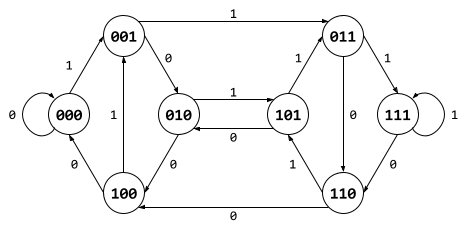
\includegraphics[scale=0.5]{graphics/b24_graph.png}
\caption{$B(2,4)$ Graph}
\label{fig:$B(2,4)$ Graph}
\end{figure}

\begin{property}
\normalfont By following an Eulerian circuit through a $B(k,n-1)$ graph, and recording the label of each edge as it is visited, one gets a $B(k,n)$ sequence. Furthermore, the set of sequences constructed by taking all Eulerian circuits in the $B(k,n-1)$ graph is identical to the set of $B(k,n)$ sequences. This fact is key in creating a generating algorithm. 
\end{property}

\begin{property}
\normalfont An Eulerian traversal of a de Bruijn graph is a circuit.
\end{property}
\begin{proof}
The indegree of each edge of a de Bruijn graph equals its outdegree (Property 2.3). Let $v$ be the start vertex of the Eulerian traversal. For $v$ to have been traversed to, on each occasion, it must have first been traversed away from. Thus, once all incoming edges to $v$ have been traversed, the outgoing edges necessarily have also been traversed. Therefore, if it is not the case that an incoming edge to $v$ is the final edge to be traversed (making the traversal a circuit), then the traversal cannot be Eulerian. 
\end{proof}


\section{A Generating Algorithm}
\subsection{Overview}
The following method will generate all de Bruijn sequences of $B(k,n)$ for given values of $k$ and $n$ in two parts: first, generate the corresponding de Bruijn graph; second, traverse through it in all ways which visit each edge exactly once. 

\subsection{Constructing the Graph}
The $B(k,n)$ graph will be represented by an adjacency matrix\footnote{An \emph{adjacency matrix} is a boolean-valued $n$ by $n$ matrix where the indices of the rows and columns correspond to the vertices $1, \dots, n$ in the graph, and the truth-value at a coordinate $(i, j)$ depends on the existence of an edge from vertex $i$ to vertex $j$.}. The data structure of choice will be a 2-dimensional array $A_{ij}$, for $0\leq i,j \leq k^{n-1}$. This choice gives a space complexity of $O(k^{2n-2})$, which is generally unideal for sparse graphs, however we should expect time complexity to be a vastly larger bottleneck for most values of n and k. This choice gives a time complexity for accessing any element of the matrix of O(1). \par
Each vertex (a value in base-k) corresponds to the index of that value in decimal. Then whether one vertex points to another (or the same) depends on if the rightmost $n-1$ characters of the row index are the same as the leftmost $n-1$ characters of the column index (in the spirit of the example described under Property 2.5). The adjacency matrix corresponding to the $B(2,3)$ graph is pictured in Figure 3, and can be verified by examining Figure 1.

\begin{figure}[ht!]
\centering
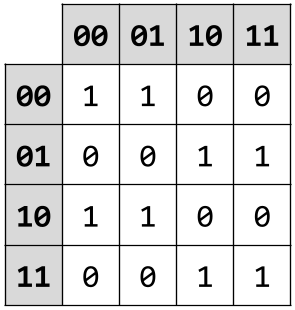
\includegraphics[scale=0.4]{graphics/b23_adjmatrix.png}
\caption{$B(2,4)$ Adjacency Matrix}
\label{fig:$B(2,4)$ Adjacency Matrix}
\end{figure}

\subsection{Traversing the Graph}
From properties 2.7 and 2.8, we conclude that finding all B(k,n) sequences is equivalent to finding all distinct traversals of the B(k,n) graph which visit each edge once. This will be implemented by recursively traversing through the graph and identifying all traversals which meet that criterion, similar to a depth-first search. Each time a vertex is reached, there are two cases to consider:\newline
\emph{Case}: The vertex has non-traversed outgoing edges.\newline
Then the edge with the label of lowest numerical value is followed, that edge is noted as visited, and it's label is appended to a list.\newline
\emph{Case}: The vertex has no non-traversed outgoing edges.\newline
Then, if the list is length $k^{n}$, an Eulerian circuit has been completed, and the list is a de Bruijn sequence, so it is stored. If the list is less than length $k^{n}$, that traversal did not complete an Eulerian circuit and the list is not stored. In either case, the rightmost character is truncated from the list, and the vertex in question returns to the previously visited one.\newline
\indent This algorithm terminates when all paths in the graph have been traversed. Implementation involves the use of some additional data structures. A $k^{n-1} \times k^{n-1}$ boolean matrix can be used to keep track of whether an edge has yet been traversed, allowing for $O(1)$ access. Something in the form of a stack data structure ought to be used to store the values of the edges which have been traversed, as this allows for $O(1)$ pushing to and popping from the list. 

\subsection{Additional Notes}
A Java implementation of an algorithm of this form is provided by myself, along with a suite of other tools pertaining to de Bruijn sequences and graphs. This code and select output files from the generating function can be found at github.com/reednel/DeBruijn. \par
In practice, it’s biggest bottleneck is neither time nor space complexity (in runtime). The problem is one of volume of data output. These sequences grow in number and length extraordinarily fast (recall Properties 2.1 and 2.2). At 1 byte/character, a file containing all $B(2,6)$ sequences would be 4 gigabytes in size. A file containing all $B(2,7)$ sequences would be 65 thousand petabytes. Changing the alphabet makes for even more radical growth. A single $B(10,10)$ sequence would be 10 gigabytes. 

\section{Applications}
De Bruijn sequences have applications in a diverse set of areas. Most notable among them may be gene sequencing in the field of genomics. The basic idea is that codons can be thought of as characters in the alphabet $A$, and a de Bruijn sequence constructed from them provides an efficient, redundancy-free series of coding sequences. \citep{peng_ji_zhao_2016} \par
Another interesting application is in (especially self working)\footnote{A \emph{self working} trick refers to one which follows a fixed procedure that does not depend on circumstance or skill.} card magic. For example, one might leverage the binary color options to order the deck in a $B(2,n)$ de Bruijn sequence. The spectator then draws n consecutive cards and recites their colors, on order. With this information and a bit of memorization ahead of time, the performer is able to identify exactly where in the sequence the spectator drew from, and thus what the values of their cards are. A strength of this trick is that one can cut the deck \emph{ad infinitum} without ever breaking the sequence. Out of personal curiosity, the I have explored the possibility of strengthening this type of trick by using binary de Bruijn sequences which can be shuffled while retaining their order. The curious reader can find this work after the conclusion of the main paper. \par
For an idea of some of the other applications, de Bruijn sequences have been used in fMRI research, bit operations in computer science, and even in cracking PIN locks which accept rolling input. 


\section{Summary}
De Bruijn sequences and graphs have many interesting and not-too-complicated properties. This fact allowed me to extend my research beyond the existing literature and into a more exploratory domain. This resulted in the identification of several properties unstated in the literature, and an apparently novel generating algorithm. \par
While applications for de Bruijn sequences extend beyond what was discussed in section 4, none appear to be too grand or significant. The diversity of applications is perhaps more notable than the applications themselves. 


\bibliographystyle{plain}
\bibliography{references}


\newpage
\section{Shuffling of Binary de Bruijn Sequences}

\subsection{Shuffling}
This extra work explores special binary de Bruijn sequences which have the property that after undergoing a perfect shuffle, they retain their original order. For brevity, we will say a binary de Bruijn sequence \emph{shuffles} if and only if it has this property. Furthermore, in this section, perfect shuffle\footnote{Concerning playing cards, a perfect shuffle (in or out) corresponds to a perfect \emph{Faro shuffle}. In practice, it would take much skill to reliably execute the Faro shuffle perfectly.} refers to a perfect \emph{in-shuffle} or perfect \emph{out-shuffle}.\par
Let $n$ be the length of a sequence, and $i$ denote the index of each element in the sequence, for $0\leq i\leq n-1$. An in-shuffle reorders the elements of the sequence according to the following rule:
\begin{equation}
     \begin{array}{lr}
        i \rightarrow 2i+1, & \text{for } 0 \leq i < \frac{n}{2}  \\
        i \rightarrow 2i-n, & \text{for } \frac{n}{2} \leq i < n 
    \end{array} 
\end{equation}
\begin{example}
Take a sequence to be of length 10. An in-shuffle reorders it’s indices as follows (underlining for visual aid):\\
\centerline{$\underline{01234}56789 \rightarrow 5\underline{0}6\underline{1}7\underline{2}8\underline{3}9\underline{4}$}
\end{example}

Let $n$ be the length of a sequence, and $i$ denote the index of each element in the sequence, for $0\leq i\leq n-1$. An out-shuffle reorders the elements of the sequence according to the following rule:
\begin{equation}
     \begin{array}{lr}
        i \rightarrow 2i, & \text{for } 0 < i < \frac{n}{2}  \\
        i \rightarrow 2i-n+1, & \text{for } \frac{n}{2} \leq i < n 
    \end{array} 
\end{equation}
\begin{example}
Take a sequence to be of length 10. An out-shuffle reorders it’s indices as follows (underlining for visual aid):\\
\centerline{$\underline{01234}56789 \rightarrow \underline{0}5\underline{1}6\underline{2}7\underline{3}8\underline{4}9$}
\end{example}

\subsection{Properties}
\begin{property}
\normalfont For a given n, it’s not true that all $B(2,n)$ sequences shuffle.\footnote{It would be of interest to prove that for all n, there exists a $B(2,n)$ sequence that shuffles.}
\end{property}

\begin{property}
\normalfont Of sequences that shuffle, only certain rotations do. 
\end{property}

\subsection{Algorithms}
I have written a suite of tools to identify $B(2,n)$ sequence that shuffle. For the reason that these algorithms are simpler and less interesting than the generating algorithm provided in the paper, they are left out here. Similar to the generating algorithm, the Java code for these tools can be found on github.com/reednel/DeBruijn. Below are some results from a function which checks each rotation of each sequence provided by the generator, and returns those which out-shuffle.

\begin{figure}[ht!]
\centering
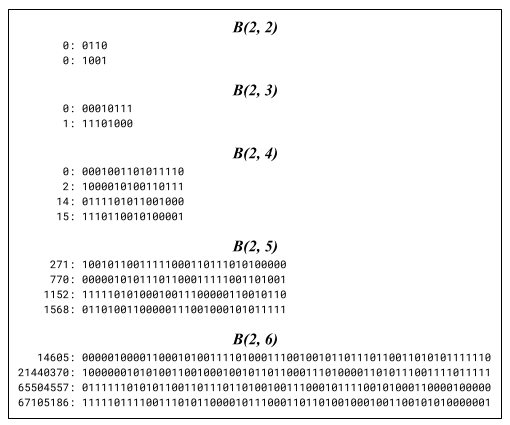
\includegraphics[scale=0.7]{graphics/b_outshuffles.png}
\caption{Sample out-shuffling de Bruijn sequences}
\label{}
\end{figure}


\end{document}
